%==============================================================================
% introduction.tex
%==============================================================================

\chapter{Introduction}
\label{chap:introduction}

Intervals \cite{Matsakis2009b} are a new, higher-level primitive for
parallel programming with which programmers directly construct the
program schedule. They are under active development at ETH Zürich as
part of the PhD research of Nicholas Matsakis \cite{Matsakis2010}.

The intervals implementation in Java uses a work-stealing scheduler in
which a worker that runs out of work tries to ``steal'' work from
others. The scope of this thesis is to improve the efficiency of the
intervals scheduler.


\section{Intervals}
\label{sec:intro-intervals}

Traditional primitives for synchronizing multi-threaded programs, such
as semaphores and barriers, are low-level and dangerous to use. They
require careful attention to implementation details to achieve good
performance, and they are prone to errors, particularly deadlocks and
race conditions.

Intervals are a higher-level alternative that make parallel
programming safer while retaining the flexibility and efficiency of
threads. In the Intervals model, users create lightweight tasks and
order them using explicit \emph{happens before} relations
\cite{Lamport1978}. Users need not specify when a thread should block
or acquire a lock. Instead they specify when a task should execute
relative to other tasks, and what locks it should hold when it
executes. The details of making this schedule pass are left to the
runtime system.

The intervals API supports arbitrary \emph{happens before} relations
making the model very flexible. Intervals can be used to emulate
existing thread primitives \cite{Matsakis2009b}, but they can also be
used to easily create program schedules for which no standard thread
primitives exist, such as peer-to-peer synchronization.

One of the primary goals in developing intervals is that program
errors should not lead to deadlocks. This includes both misuse of the
APIs but also miscellaneous errors which causes tasks to abort
unexpectedly, such as dereferencing a null pointer
\cite{Matsakis2009}. A further goal is that an error in one task
should prevent other, dependent tasks from executing
\cite{Matsakis2010a}.

\subsection{Model}
\label{sec:intro-intervals-model}

Intervals are first-class objects in the programming language that
represent the slice of program time used to execute a parallel
task. Intervals are structured hierarchically in a tree. The root of
the interval tree represents the entire program execution. Program
execution itself begins in a child of the root interval.

The conceptual model for intervals consists of points in time ordered
by a \emph{happens before} relation. In the model, an interval
\lstinline|i| consists of a pair of points -- \lstinline|i.start| and
\lstinline|i.end| -- called the start and end point. The start point
represents the moment when the interval begins execution. The end
point represents the moment when the interval's task is
completed. Programmers may introduce arbitrary ordering constraints by
adding \emph{happens before} edges between the start or end points of
different intervals. An edge \lstinline|p1 $\rightarrow$ p2| indicates
that the point \lstinline|p1| must occur before the point
\lstinline|p2|. It also indicates that any memory writes which
\emph{happen before} \lstinline|p1| must be visible to
\lstinline|p2|.

\begin{figure}[htb]
  \centering
  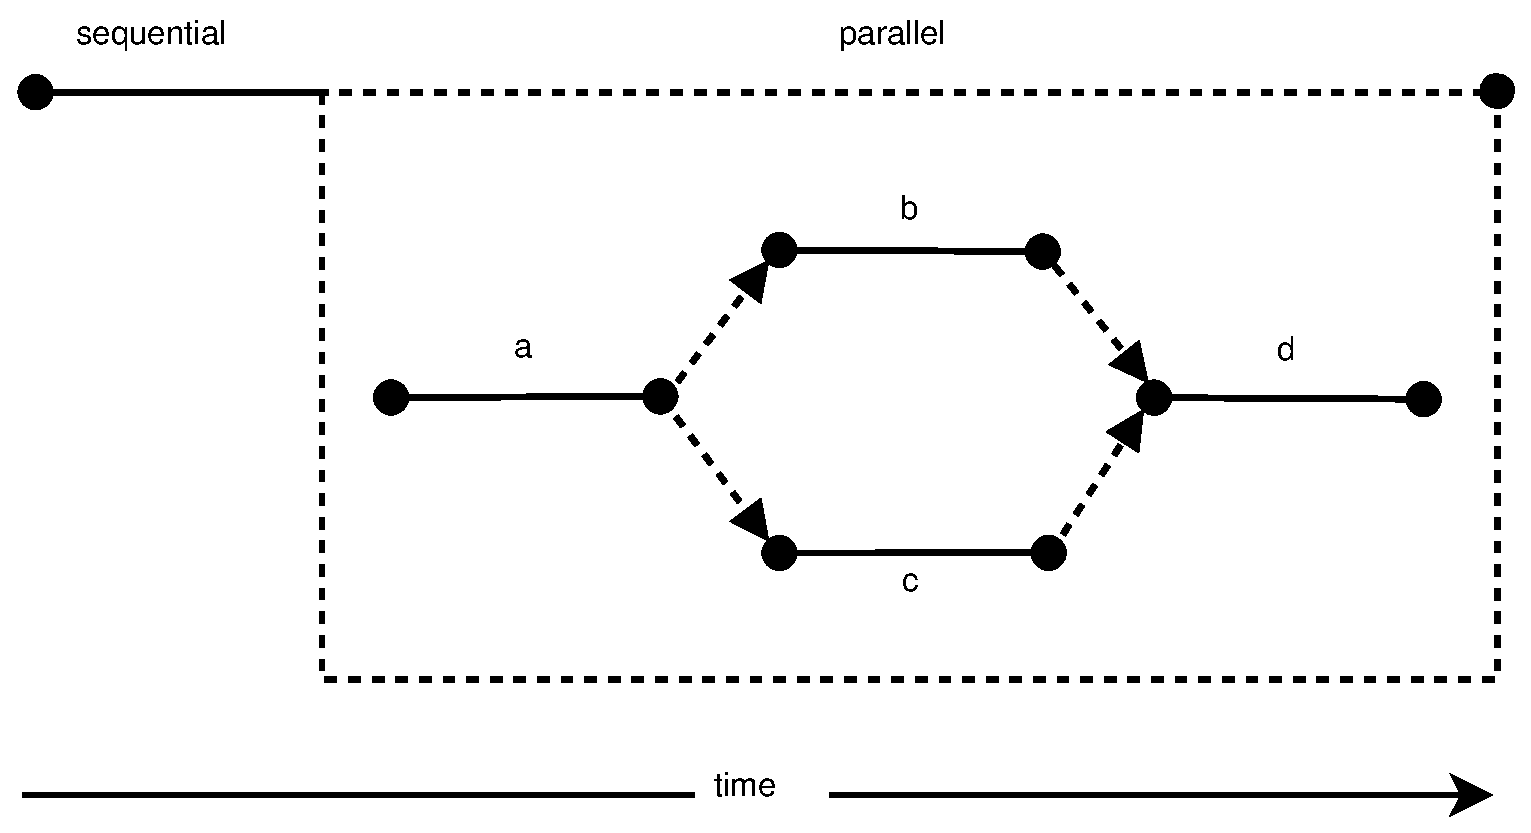
\includegraphics[width=0.96\textwidth]{introduction/interval-graph}
  \caption[Example interval graph]{Example interval graph: Showing an
    interval and its subintervals \lstinline|a|, \lstinline|b|,
    \lstinline|c| and \lstinline|d|.}
  \label{fig:interval-graph}
\end{figure}

An interval can be associated with one or more locks. The intervals
runtime will automatically acquire those locks before the interval's
start point occurs and release them after its end point has occurred.

When an interval executes, it begins by invoking the sequential method
\lstinline|run()|. \lstinline|run()| may either perform the task
directly or create a number of subintervals to achieve the task in
parallel. These subintervals begin to execute once the
\lstinline|run()| method has completed and they are ready to run. A
subinterval is ready to run when it could execute without violating
the \emph{happens before} relation. It will be executed when it is
ready and acquired all its locks.

The interval model can be depicted as a graph, as shown in Figure
\ref{fig:interval-graph}. The graph contains a single interval with
four subintervals, \lstinline|a|, \lstinline|b|, \lstinline|c| and
\lstinline|d|. The start and end points of each interval are
represented as opaque circles. The subintervals of an interval are
enclosed in a dashed box. This dashed box is omitted for leaf
intervals.

The dashed edges connecting different points indicate user-specified
additions to the \emph{happens before} relation. For example, the end
of \lstinline|a| \emph{happens before} the start of \lstinline|b| and
\lstinline|c| and the ends of \lstinline|b| and \lstinline|c| both
\emph{happen before} the start of \lstinline|d|.

\subsection{Java API}
\label{sec:intro-intervals-java-api}

In the Java API, intervals are represented as instances of the
abstract class \lstinline|Interval| (Listing
\ref{lst:interval-class}). \lstinline|Interval| provides immutable
fields to access the interval's start point, end point, and parent,
along with an abstract \lstinline|run()| method which must be
redefined in a concrete subtype.

\begin{lstlisting}[
  style=Float, 
  caption={[\lstinline{Interval} class] \lstinline{Interval}: Serves as the base class for all intervals},
  label=lst:interval-class
]
public abstract class Interval {
  public final Interval parent;
  public final Point start;
  public final Point end;

  protected abstract void run();
}
\end{lstlisting}

Listing \ref{lst:interval-graph} contains Java code which uses the
Intervals API to construct the graph shown in Figure
\ref{fig:interval-graph}.

\begin{lstlisting}[
  style=FloatNumbers, 
  caption={[Intervals Java API example] Code to produce the sample interval graph shown in Figure \ref{fig:interval-graph}},
  label=lst:interval-graph
]
public class ExampleInterval extends Interval {
  public ExampleInterval(Dependency dep, String name) {
    super(dep, name);
  }
  
  protected void run() {
    // Task
  }
  
  public static void main(String[] args) {
    Intervals.inline(new VoidInlineTask() { //*\label{lst:interval-graph-inline-start}
      public void run(Interval start) {
        Interval a = new ExampleInterval(start, "a"); //*\label{lst:interval-graph-new-start}
        Interval b = new ExampleInterval(start, "b");
        Interval c = new ExampleInterval(start, "c");
        Interval d = new ExampleInterval(start, "d"); //*\label{lst:interval-graph-new-end}
        
        Intervals.addHb(a, b); //*\label{lst:interval-graph-add-hb}
        Intervals.addHb(a, c);
        Intervals.addHb(b, d);
        Intervals.addHb(c, d);
        Intervals.schedule(); //*\label{lst:interval-graph-schedule}
      }
    }); //*\label{lst:interval-graph-inline-end}
  }
}
\end{lstlisting}

\subsubsection{Creating Intervals}
\label{sec:intro-intervals-creating-intervals}

To start program execution, the programmer has to create a new child
of the root interval. One could for example use an inline interval to
do so. Inline intervals execute a task during the current interval and
do not return until the task has completed.

Lines \ref{lst:interval-graph-inline-start} --
\ref{lst:interval-graph-inline-end} create the inline subinterval
\lstinline|start| by providing an anonymous task class redefining its
\lstinline|run()| method. \lstinline|start| has four subintervals,
\lstinline|a|, \lstinline|b|, \lstinline|c| and \lstinline|d|. They
are created on Lines \ref{lst:interval-graph-new-start} --
\ref{lst:interval-graph-new-end} and are normal, non-blocking
intervals.

\subsubsection{Scheduling Intervals}
\label{sec:intro-intervals-scheduling-intervals}

Newly constructed intervals become eligible for execution once the
\lstinline|schedule()| method is invoked, as shown on Line
\ref{lst:interval-graph-schedule} in Listing
\ref{lst:interval-graph}. This gives the user the opportunity to
construct any required dependencies or perform other
initialization. For example, adding the edge
\lstinline|a $\rightarrow$ b| on Line \ref{lst:interval-graph-add-hb}
would be unsafe if \lstinline|b| could begin immediately, as it would
be possible that \lstinline|b.start| had already occurred before the
call to \lstinline|addHb()| could add the new dependency.

Explicit calls to \lstinline|schedule()| are unusual, however. This is
because the runtime automatically invokes \lstinline|schedule()| when
the \lstinline|run()| method of an interval returns.


\section{Work-Stealing Scheduler}
\label{sec:intro-work-stealing-scheduler}

The implementation of intervals for Java makes use of a work-stealing
scheduler similar to those found in Cilk \cite{Blumofe1995,
  Frigo1998}, Java 7 \cite{Lea2000, Lea2000a, Lea2004, Lea2006}, Intel
Threading Building Blocks (TBB) \cite{Reinders2007, Contreras2008}, or
Microsoft Task Parallel Library \cite{Leijen2009} but extended to
support locks and happens before edges.

A work-stealing scheduler employs a fixed number of threads called
workers. Each worker has a local double-ended queue, or deque, to
maintain its own pool of ready tasks from which it obtains work. When
a worker finds that its pool is empty, it becomes a thief and steals a
task from the pool of a victim worker chosen at random.

To obtain work, a worker pops the ready task from the bottom of its
deque and executes it. If the task terminates, the worker goes back to
the bottom of its deque to pop off another task upon which it can
work. When assigning a new task to a worker, the worker pushes the
newly ready task onto the bottom of its deque. Thus, so long as a
worker's deque is not empty, the worker manipulates its deque in a
LIFO (stack-like) manner.

When a worker tries to obtain work by popping a task off the bottom of
its deque and it finds that it is empty, then the worker becomes a
thief. It picks a victim worker at random and attempts to obtain work
by removing the task at the top of the victim worker's deque. If the
victim worker's deque is empty, then the thief picks another victim
worker and tries again until it finds a victim whose deque it
non-empty. At which point the thief continues to work on the stolen
task as described above. Since steals take place at the top of the
victim's deque, stealing operates in a FIFO manner.

Accessing the run queues at different ends offers several advantages
\cite{Frigo1998}:

\begin{itemize}
\item It reduces contention by having stealers operate on the opposite
  side of the deque as owners
\item It exploits the property of recursive divide-and-conquer
  algorithms of generating ``large'' tasks early. Thus, an older
  stolen task is likely to provide a larger unit of work, leading to
  further recursive decompositions by the stealing worker.
\item Stealing a task also migrates its future workload, which helps
  to increase locality.
\end{itemize}

The assignment of tasks to workers for execution is done in a provably
efficient manner \cite{Blumofe1995, Blumofe1999}.


\section{Overview}
\label{sec:intro-overview}

In \autoref{part:locality} of the thesis we implement and analyze
locality-aware scheduling of intervals. Locality-aware scheduling
allows each interval to be given an affinity for a place, and when a
worker belonging to a certain place obtains an interval, it gives
priority to the intervals with affinity for the place \cite{Acar2002,
  Guo2010}.

In the non-blocking work-stealing algorithm, the deques are
implemented with non-blocking synchronization \cite{Arora2001}. The
current deque implementation of intervals however uses a lock when
trying to steal. As a separate effort, we designed and explored
alternative non-blocking queue implementations with the aim to improve
scheduling performance (see \autoref{part:queues}).

\todo{Rewrite overview}

% The goal of the thesis is to improve the implementation of the
% intervals scheduler and it is divided into two parts.

% \subsubsection{\autoref{part:locality}. Locality-Aware Work-Stealing}

% In \autoref{part:locality} of the thesis we implement and analyze
% locality-aware scheduling of intervals. Locality-aware scheduling
% allows each interval to be given an affinity for a place, and when a
% worker belonging to a certain place obtains an interval, it gives
% priority to the intervals with affinity for the place \cite{Acar2002,
%   Guo2010}.

% \subsubsection{\autoref{part:queues}. Work-Stealing Queue
%   Implementations}

% The original work-stealing algorithm uses non-blocking algorithms to
% implement queue operations \cite{Arora2001}. However, the current
% deque implementation of intervals uses a lock when trying to steal. In
% \autoref{part:queues} of this thesis we explore alternative
% non-blocking queue implementations and compare them to the current
% one.

%%% Local Variables: 
%%% mode: latex
%%% TeX-master: "thesis"
%%% End: 
